% !TEX encoding = UTF-8 Unicode
% лекции 3-4, 20 февраля 2016
% вопросы 6-8
% 6. Задача Коши для одномерного волнового уравнения (колебания бесконечной струны). Вывод формулы Даламбера при помощи транспортного уравнения. Свойства решения. Волновые конусы. Конечная скорость распространения волн. Передний и задний фронт волны.
% 7-8. Канонический вид уравнений в частных производных второго порядка, их классификация.

\subsection{Задача Коши для одномерного волнового уравнения}
Будем считать, что струна настолько длинная, что краевыми эффектами того, что струна зажата на концах, можно пренебречь. То есть, что струна просто колеблется в соответствии с нашим волновым уравнением. Волновое уравнение --- один из тех редких случаев, когда можно получить общую формулу решения.
Решение выведем двумя способами.
\subsubsection{Вывод решения при помощи транспортного уравнения}
\begin{gather*}
	u_{tt} - v^2 u_{xx} = (\pder{t} - v \pder{x}) \underbrace {(\pder[u]{t} + v \pder[u]{x})}_{= w} = 0, \\
 	\pder[w]{t} - v \pder[w]{x} = 0.
\end{gather*}

Получили однородное транспортное уравнение, его решение мы знаем:
\begin{gather*}
	w(t,x) = \psi (x + vt),\quad \psi (x) = w(0,x) \\
	\pder[u]{t} + v \pder[u]{x} = \psi (x + vt)		
\end{gather*}

Получили неоднородное транспортное уравнение, его решение мы тоже знаем:
\begin{gather*}
	u(t,x) = u_0 (x - vt) + \int \limits_0^t \psi(x + vs - v(t-s)) ds = u_0 (x - vt) + \int \limits_0^t \psi (x - vt + 2vs) ds, \\
	\text{сделаем замену }y = x - vt + 2vs, \text{ тогда} \\
\end{gather*}
\begin{equation}
    u(t,x) = u_0 (x - vt) + \frac {1} {2v} \int \limits_{x-vt}^{x+vt} \psi (y) dy
\label{wavehomans}
\end{equation}
% Красивый номер страницы - это специально? :)
\begin{exercise}
При каких $\varphi$ и $\psi$ $\eqref{wavehomans}$ --- решение $\eqref{waveequation}$? (Ответ: $\varphi \in C^2$, $\psi \in C^1$)
\end{exercise}

\begin{theorem} Пусть $\varphi \in C^2(\real)$ и $\psi \in C^1(\real)$. Тогда
$$ u(t, x) = \varphi (x - vt) + \frac {1} {2v} \int \limits_{x - vt}^{x+vt} \psi (y) dy$$
--- решение одномерного волнового уравнения.
\end{theorem}

Поставим задачу Коши для волнового уравнения:

\begin{align}
    \begin{cases} 
        u_{tt} - v^2 u_{xx} = 0, \\
        u (0, x) = u_0 (x), \\
        u_t(0,x) = v_0 (x).
    \end{cases}
\label{wavecauchy}
\end{align}
%
Найдем решение задачи Коши. Подставляя $(0,x)$ в общее решение, получаем $$ u_0(x) = \varphi(x) .$$ Найдём $v_0(x)$:
\begin{gather*}
	u_t(0,x) = v_0(x) = \frac {1} {2v} (v \psi (x + vt) + v \psi (x - vt)) \Bigg\rvert_{t = 0} - v \varphi' (x)
	= \psi(x) - v \varphi'(x), \\
	\psi(x) = v_0(x) + v u'_0(x).
\end{gather*}
Таким образом,
\begin{align*}
	u(t,x) &= u_0(x-vt) + \frac {1} {2v} \int \limits_{x-vt}^{x+vt} v_0(y) + vu'_0(y)dy \\
	&= u_0(x-vt) + \frac {u_0(x+vt) - u_0(x-vt)} { 2} + \frac {1} {2v} \int \limits_{x-vt}^{x+vt} v_0(y)dy.
\end{align*}
Отсюда легко получаем формулу Д'Аламбера
\begin{equation}
	u(t,x) = \frac {u_0(x+vt) + u_0(x-vt)} { 2} + \frac {1} {2v} \int \limits_{x-vt}^{x+vt} v_0(y)dy.
\label{wavedalembert}
\end{equation}

Сформулируем теорему:
\begin{theorem} Пусть $u_0 \in C^2(\real)$ и $v_0 \in C^1(\real)$, тогда формула Д'Аламбера $\eqref{wavedalembert}$ --- единственное классическое решение задачи Коши для уравнения колебания бесконечной струны.
\end{theorem}

\begin{example}
Пусть $t$ --- время, $x$ --- координата вдоль струны. Предположим, на струне в точке $x_0$ сидит муравей. (Мировая линия объекта - траектория его движения в координатах пространства и времени) Пусть для простоты он не двигается. $x(t)$ - мировая линия, $v_0 = 0$. $x + vt = const$ и $x -vt = const$ - характеристические функции.

%TODO: рисунок про конусы
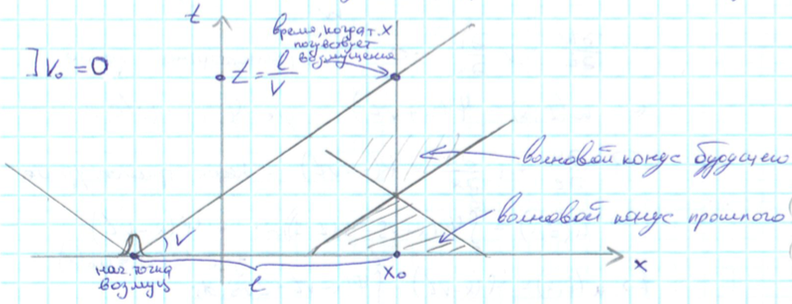
\includegraphics[scale=0.5]{part2.1.png}

Допустим, кто-то в точке $(x0-l)$ ударил по струне, для простоты пусть этот кто-то её отклонил, но не придал никакой начальной скорости ($v_0 = 0$, $u_0 \neq 0$). Когда муравей узнает о том, что что-то произошло? В момент времени $ t = \frac {l} {v}$, где $l$ - расстояние от муравья до источника возмущения, $v$ - модуль скорости распространения возмущения. Будем считать, что профиль возмущения локализован около точки, тогда профиль распространяется вперёд и назад: бегут две волны. Если бы щелчок по струне был локализован в одной точке (тогда это не было бы классическим решением!), то муравей почуствовал бы фронт волны только на мгновение. Волновой конус будущего для конкретных точки, в которой произошло мгновенное возмущение, и времени -- это множество точек, которых достигнет возмущение в будущем. Волновой конус прошлого для конкретных точки, в которой сидит муравей, и времени -- это множество таких точек, возмущение в которых в прошлом будет почувствовано муравьем. Границы конусов зависят от скорости распространения возмущения.
Интегрируем по содержимому конуса прошлого. Задав скорость муравью, можно повлиять на содержимое конуса будущего.
\end{example}

{\small А что будет в трёхмерном случае? Распространение сферических волн. В отличие от формулы Д'Аламбера, не будет разницы между начальным возмущением с некоторой начальной скоростью и без неё. То есть, сферические фронты будут доходить от каждой точки волны. Сначала дойдёт передний фронт, потом задний.

А в двумерном? Распространение цилиндрических волн. Пример - берём удочку с поплавком, идём на пруд без течения. Забрасываем удочку, бросаем далеко от поплавка камушек. Получится примерно точечное возмущение. В какой-то момент передний фронт дойдёт до поплавка и он начнёт дёргаться. Волна пройдёт, а поплавок продолжит свои колебания, теоретически - бесконечно долго. То есть, заднего фронта не будет.}

% Ч Т О ?
TODO: написать нормально про конусы

\subsubsection{Вывод решения при помощи замены переменных}
$$u_{tt} - v^2 u_{xx} = 0$$
Сделаем замену $(t, x) \to (\xi, \eta)$:
$$ \xi = x + vt, \quad \eta = x - vt.$$
\begin{align*}
	u_x &= u_{\xi} \xi_x + u_{\eta} \eta_x = u_{\xi} + u_{\eta}, \\
	u_t &=  u_{\xi} \xi_t + u_{\eta} \eta_t = v u_{\xi} + v u_{\eta}, \\
	u_{xx} &= u_{x\xi} \xi_x + u_{x\eta} \eta_x = u_{\xi\xi} + u_{\eta\xi} + u_{\xi\eta} + u_{\eta\eta}  =  u_{\xi\xi} + 2 u_{\xi\eta} + u_{\eta\eta}, \\
	u_{tt} &= u_{t\xi} \xi_t + u_{t\eta} \eta_t = v^2 (u_{\xi\xi} - u_{\eta\xi}) - v^2 (u_{\xi\eta} - u_{\eta\eta}) = v^2 (u_{\xi\xi} - 2u_{\xi\eta} + u_{\eta\eta}). \\
	\square_v u &= v^2 u_{\xi\xi} - 2v^2 u_{\xi\eta} + v^2 u_{\eta\eta} - v^2 u_{\xi\xi} - 2v^2 u_{\xi\eta} - v^2 u_{\eta\eta} = 0, \\
	u_{\xi\eta} &= 0, \quad u_{\xi} = F(\xi), \\
	u &= \int F(\xi) d\xi = \varphi (\xi) + \psi (\eta). \\
\end{align*}
Таким образом,
$$ u = \underbrace {\varphi (x+vt)}_{\text{волна направо}} + \underbrace {\psi (x-vt)}_{\text{волна налево}}.$$

Решим задачу Коши $\eqref{wavecauchy}$:
\begin{gather*}
	\begin{cases}
		u(0,x) = u_0(x) = \varphi(x) + \psi(x), \\
		u_t(0,x) = v_0(x) = v \varphi'(x) - v \psi'(x),
	\end{cases}
	\begin{cases}
		\psi(x) = u_0(x) - \varphi(x), \\
		v \varphi'(x)  - vu'_0(x) + v \varphi'(x) = v_0(x).
	\end{cases} \\
	\varphi'(x) = \frac {1} {2v} (v_0(x) + vu'_0(x)), \quad 	\varphi(x) = \frac {1} {2v} \int \limits_0^x v_0(y) + vu'_0(x) \,dy + C, \\
	\psi(x) = u_0 - \frac {1} {2v} \int \limits_0^x v_0(y) + vu'_0(y) \,dy - C,
\end{gather*}
Тогда
\begin{align*}
	u(t,x) &= \frac {1} {2v} \int \limits_0^{x+vt} v_0(y) + vu'_0(y) + C + u_0(x-vt) -  \frac {1} {2v} \int \limits_0^{x-vt} v_0(y) + vu'_0(y) dy - C \\
		&= u_0(x-vt) + \frac {1} {2v} \int \limits_{x-vt}^{x+vt} v_0(y) + v u'_0(y) dy.
\end{align*}
Отсюда легко получается та же самая формула Д'Аламбера \eqref{wavedalembert}:
\begin{equation*}
	u(t,x) = \frac {u_0(x+vt) + u_0(x-vt)} {2} + \frac {1} {2v} \int \limits_{x-vt}^{x+vt} v_0(y)dy.
\end{equation*}

% !TEX encoding = UTF-8 Unicode
% лекции 3-4, 20 февраля 2016
% вопросы 6-8
% 6. Задача Коши для одномерного волнового уравнения (колебания бесконечной струны). Вывод формулы Даламбера при помощи транспортного уравнения. Свойства решения. Волновые конусы. Конечная скорость распространения волн. Передний и задний фронт волны.
% 7-8. Канонический вид уравнений в частных производных второго порядка, их классификация.

\subsection{Приведение уравнений второго порядка к каноническому виду в случае двух независимых переменных}

Ранее мы получили решение одномерного волнового уравнения путём замены переменных. Нет ли способа, позволяющего получить замену переменных, приводящую уравнение к некоторому "красивому" виду в общем случае?

Рассмотрим линейное дифференциальное уравнение в частных производных второго порядка с нелинейными коэффициентами:
$$ a u_{xx} + 2bu_{xy} + c u_{yy} + d_1 u_x + d_2 u_y + d_3 u = f.$$
Будет приятно иметь локально обратимое преобразование координат (якобиан преобразования $\neq$ 0). Рассмотрим гладкую замену 
$$(x,y) \rightarrow (\xi, \eta).$$
Применяя правило дифференцирования сложной функции, пересчитаем производные в новых координатах:
\begin{align*}
	u_x &= u_\xi \xi_x + u_\eta \eta_x, \\
	u_y &= u_\xi \xi_y + u_\eta \eta_y, \\
	u_{xx} &= u_{\xi x} \xi_x + u_{\eta x} \eta_x + u_\xi \xi_{xx} + u_\eta \eta_{xx} = u_{\xi \xi} \xi^2_x + 2u_{\xi \eta} \xi_x \eta_x + u_{\eta \eta} \eta^2_x + u_\xi \xi_{xx} + u_\eta \eta_{xx}, \\
	u_{yy} &= u_{\xi y} \xi_y + u_{\eta y} \eta_y + u_\xi \xi_{yy} + u_\eta \eta_{yy} = u_{\xi \xi} \xi^2_y + 2u_{\xi \eta} \xi_y \eta_y + u_{\eta \eta} \eta^2_y + u_\xi \xi_{yy} + u_\eta \eta_{yy}, \\
	u_{xy} &= u_{\xi \xi} \xi_x \xi_y + u_{\xi \eta} (\xi_x \eta_y + \xi_y \eta_x) + u_{\eta \eta} \eta_x \eta_y + u_\xi \xi_{xy} + u_\eta \eta_{xy}.
\end{align*}
Подставим в наше уравнение:
\begin{align*}
	u_{\xi \xi} & (a \xi^2_x + 4b \xi_x \xi_y + c \xi^2_y) + \\
	u_{\eta \eta} & (a \eta^2_x + 4b \eta_x \eta_y + c \eta^2_y) +\\
	2 u_{\xi \eta} & (a \xi_x \eta_x + 4b \xi_x \eta_y + c \xi_y \eta_y) + \\
	u_\xi & (a \xi_{xx} + 2b \xi_{xy} + c \xi_{yy} + d_1\xi_x + d_2 \xi_y) + \\
	u_\eta & (a \eta_{xx} + 2b \eta_{xy} + c \eta_{yy} + d_1 \eta_x + d_2 \eta_y) = f.
\end{align*}

Получили
$$\underbrace {A u_{\xi \xi} + 2B u_{\xi \eta} + C u_{\eta \eta}}_{\text{новая главная часть}} + \text{ч.н.п.} = f,$$
где \begin{align*}
	A &= a \xi^2_x + 4b \xi_x \xi_y + c \xi^2_y, \\
	B &= a \xi_x \eta_x + 4b \xi_x \eta_y + c \xi_y \eta_y, \\
	C &= a \eta^2_x + 4b \eta_x \eta_y + c \eta^2_y.
\end{align*}

Замечаем, что $A$ и $C$ имеют очень похожую структуру. Нельзя ли оставить в главной части только смешанную производную? Посмотрим на систему
\begin{align*}
	\begin{cases*}
	a \xi^2_x + 4b \xi_x \xi_y + c \xi^2_y = 0, \\
	a \eta^2_x + 4b \eta_x \eta_y + c \eta^2_y = 0.
	\end{cases*}
\end{align*}
Если решение этой системы даст нам локально обратимое преобразование координат, то цель достигнута. Второе уравнение это первое (с точностью до замены переменной) так что можно рассматривать только его. Это квадратичная форма, значит,
$$ a (\xi_x - \Lambda^+ \xi_y)(\xi_x + \Lambda^- \xi_y) = a \xi^2_x - a(\Lambda^+ + \Lambda^-)\xi_x \xi_y + a \Lambda^+ \Lambda^- \xi_y^2 =  0.$$
Значит,
\begin{align*}
	\begin{cases*}
		\Lambda^+ + \Lambda^- = - \frac {2b} {a}, \\
		\Lambda^+ \Lambda^- = \frac {c} {a}.
	\end{cases*}
\end{align*}
Можно сказать, что $\Lambda^+$ и $\Lambda^-$ это корни уравнения
$$a \Lambda^2 + 2b \Lambda + c = 0,$$
откуда можно заключить, что
$$ \Lambda^{\pm} = - \frac {b} {a} \pm \sqrt{\frac {b^2} {a^2} - \frac {c} {a}} = \frac {1} {a} (-b \pm \sqrt{b^2 - ac}).$$
Обозначим $$M = \begin{pmatrix} a & b \\ b & c \\\end{pmatrix}.$$
Тогда 
\begin{enumerate}
	\item если $\det M =  ac - b^2 < 0$, то уравнение называется гиперболическим и можно вывести два транспортных уравнения:
	\begin{gather*}
		\xi_x - \frac {1} {a} (-b + \sqrt{b^2 - ac}) \xi_y = 0, \\
		\eta_x - \frac {1} {a} (-b - \sqrt{b^2 - ac}) \eta_y = 0.
	\end{gather*}
	Рассмотрим дифференциальное уравнение:  $$\xi_x = \Lambda^+ \xi_y \quad \Rightarrow \quad y_x = - \Lambda^+ (x,y)\text{ - характеристика},$$
	Пусть $\xi$ - какое-то решение, рассмотрим его на траекториях
	$$ \frac {d \xi (x, y(x))} {dx} = \xi_x + \xi_y \frac {dy} {dx} = \xi_x - \Lambda^+ \xi_y = 0,$$
	тогда решение полученного транспортного уравнения должно быть постоянным на характеристиках этого ОДУ:
	$$ \frac {d \xi (x, y(x))} {dx} = \const \quad \text{при } \frac {dy} {dx} = - \Lambda^-.$$
	% как делаете: решение определяется по этим формулам, лямбда плюс и минус - по коэффициентам. если определитель больше нуля, то есть два вещественных разных решения - лямбда плюс и лямбда минус. решаем дифференциальное уравнение с лямбда плюс и определяем функцию кси из того условия, что кси постоянна на траекториях этого диффура. если лямбда плюс - гладкая функция, то через каждую точку проходит ровно одна характеристическая линия, значит, явным образом можно определить кси. то же самое с эта: решаем уравнение dy/dx = -лямбда^-, это даёт решение второго транспортного уравнения. эти решения и будут нашей заменой переменных. тем самым гарантируется, что останется только коэффициент при u_{xi eta}. то есть для гиперболического уравнения всегда можно найти замену
	
	\item если $\det M = ac - b^2 = 0$, то уравнение называется параболическим и $$\Lambda = - \frac {b} {a} \quad \Rightarrow \quad \frac {dy} {dx} = \frac {b} {a}.$$
	Отсюда можно найти только $\xi$, в этом случае $\eta$ выбирается такая, чтобы якобиан замены не был равен нулю. 
	\begin{exercise} Показать, что в этом случае $A = 0$ и $u_{\xi \eta} = 0$.
	% A =0 ?
	\end{exercise}
	
	\item если $\det M = ac - b^2 > 0$, то уравнение называется эллиптическим и $u_{\xi \eta} =0$, $A = C \neq 0$. Корни будут комплексно сопряжёнными, а замена будет $$\xi = Re ...,\quad \eta = Im ... .$$
\end{enumerate}
	
\subsubsection{Классификация в случае двух независимых переменных}
Рассмотрим дифференциальное уравнение в частных производных второго порядка с переменными коэффициентами:
$$ \underbrace {\sum \limits_{i = 1}^2 \sum \limits_{j = 1}^2 a_{ij}(x_1, x_2) \frac {\partial^2 u} {\partial x_i \partial x_j}}_{\text{главная часть}}  + \underbrace {F(\pder[u]{x_1}, \pder[u]{x_2}, u, x_1, x_2)}_{\text{члены низшего порядка}} = 0,\quad x \in \real^2$$

Обозначим через $A$ симметричную матрицу коэффициентов $a_{ij}$.
\begin{itemize}
\item Если $\det A < 0$, то уравнение называется гиперболическим, и в некоторых координатах $(\xi, \eta)$ уравнение имеет канонический вид:
$$\frac {\partial^2 u} {\partial \xi \partial \eta} + \text{члены низшего порядка} = 0.$$
\item Если $\det A = 0$, то уравнение называется параболическим, и в некоторых координатах $(\xi, \eta)$ уравнение имеет канонический вид:
$$ \frac {\partial^2 u} {\partial \eta^2} + \text{члены низшего порядка} = 0.$$
\item Если $\det A > 0$, то уравнение называется эллиптическим, и в некоторых координатах $(\xi, \eta)$ уравнение имеет канонический вид:
$$ \frac {\partial^2 u} {\partial \xi^2} + \frac {\partial^2 u} {\partial \eta^2} + \text{члены низшего порядка} = 0.$$
\end{itemize}

В случае переменных коэффициентов $a_{ij}$ уравнение может иметь разный тип в разных областях, такие уравнения называются уравнениями переменного типа.

\subsection{Классификация уравнений второго порядка в случае многих независимых переменных}
Рассмотрим дифференциальное уравнение в частных производных второго порядка с переменными коэффициентами:
$$ \underbrace {\sum \limits_{i=1}^n \sum \limits_{j = 1}^n a_{ij} \frac {\partial^2 u} {\partial x_i \partial x_j}}_{\text{главная часть}}  + F(\pder[u]{x_1}, \pder[u]{x_2}, u, x_1, ..., x_n) = 0,\quad x \in \real^n$$

Обозначим через $A$ симметричную матрицу коэффициентов $a_{ij}$. Уравнение называется 
\begin{itemize}
\item эллиптическим, если у матрицы $A$ все собственные числа одного знака;
\item гиперболическим, если матрица $A$ имеет собственные числа разных знаков;
\item параболическим, если у матрицы $A$ есть собственное число, равное нулю.
\end{itemize}

В общем случае нужно занулить $(n^2 - n) / 2$ коэффициентов $a_{ij}$, чтобы получить диагональную матрицу. Неизвестных при этом $n$ штук. Так как
$$\frac {n^2 - n} {2} \leq n \quad \Longleftrightarrow \quad n \leq 3,$$
то при $n \leq 3$ в общем случае можно найти замену, приводящую уравнение к некоторому каноническому виду. При $n > 4$ общего способа нет.

\subsection{Примеры уравнений различных типов}

\begin{example}[Уравнение Пуассона]
$$ - \Delta u = f, \quad x \in \real^n$$
$$\begin{pmatrix}
-1 & \\
   & \ddots \\
   & & -1
\end{pmatrix}\quad \Rightarrow \quad \text{уравнение эллиптическое}.$$
\end{example}

\begin{example}[Волновое уравнение]
$$u_{tt} - v^2 \Delta u = f, \quad (t,x) \in \real^{n+1}$$
$$\begin{pmatrix}
1 & \\
   & -v^2 \\
   & & \ddots \\
   & & & -v^2
\end{pmatrix}\quad \Rightarrow \quad \text{уравнение гиперболическое}.$$
\end{example}

\begin{example}[Уравнение теплопроводности]
$$ u_t - D \Delta u = f, \quad (t,x) \in \real^{n+1}$$
$$\begin{pmatrix}
0 & \\
   & -D \\
   & & \ddots \\
   & & & -D
\end{pmatrix}\quad \Rightarrow \quad \text{уравнение параболическое}.$$
\end{example}